\section{Color Balancing}
\subsection{Cumulative Histograms}
In this section I had to calculate and plot the cumulative histograms for the R, G and B components for kodim23a.png and kodim23b.png (Figure \ref{fig:KodimImages}). These histograms can be seen in Figure \ref{fig:KodimCumHistogram}

\begin{figure}[h]
    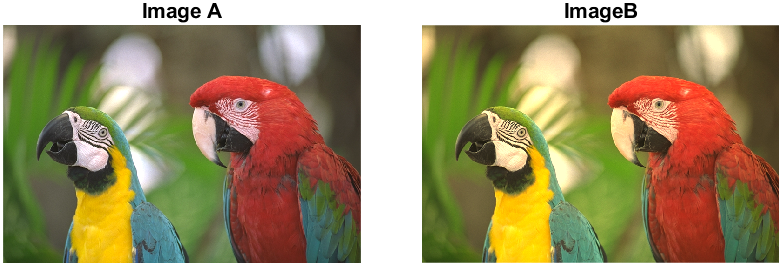
\includegraphics[width=1\textwidth]{KodimImages.png}
    \centering
    \caption{kodim23a.png and kodim23b.png}
    \label{fig:KodimImages}
\end{figure}

\begin{figure}[h]
    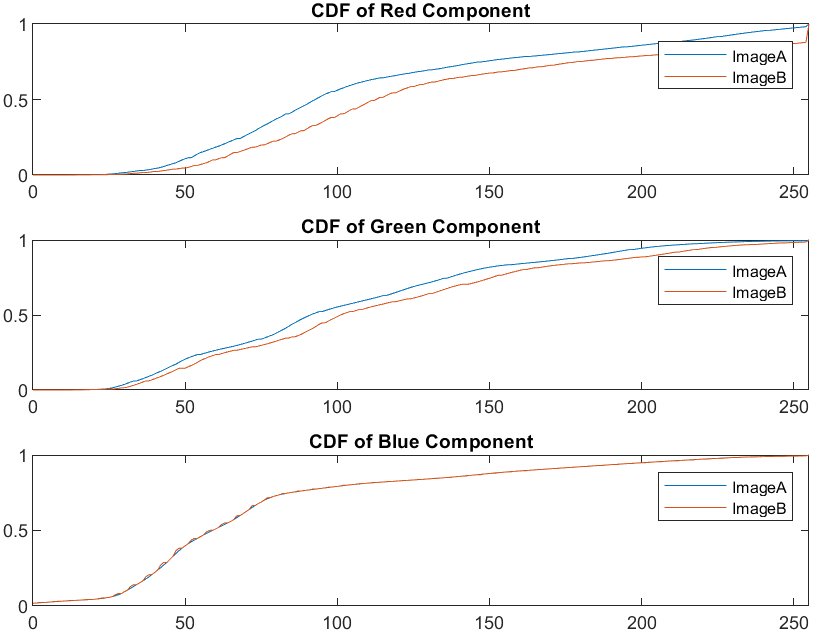
\includegraphics[width=1\textwidth]{KodimCumHistograms.png}
    \centering
    \caption{Cumulative Histograms for kodim23a and kodim23b}
    \label{fig:KodimCumHistogram}
\end{figure}

\subsection{Color Mapping Kodim23b to Kodim23a}
Using these histograms I calculated where the channel value of 150 in kodim23a got mapped to in kodim23b. These gave the values for $(R_a, G_a, B_a)^\mathrm{T}$ and $(R_b, G_b, B_b)^\mathrm{T}$. We can substitute these vectors into matrix \ref{eqn:1}, and solve the linear system to estimate the values for $(R_w, G_w, B_w)^\mathrm{T}$.

\begin{gather}
    \begin{bmatrix}
        R_a \\
        G_a \\
        B_a \\       
    \end{bmatrix}
    =
    \begin{bmatrix}
        \frac{255}{R_w} & 0 & 0 \\
        0 & \frac{255}{G_w} & 0 \\
        0 & 0 & \frac{255}{B_w}
    \end{bmatrix}
    \begin{bmatrix}
        R_b \\
        G_b \\
        B_b \\
    \end{bmatrix}
    \label{eqn:1}
\end{gather}

\begin{gather}
    \begin{bmatrix}
        150 \\
        150 \\
        150 \\       
    \end{bmatrix}
    =
    \begin{bmatrix}
        \frac{255}{R_w} & 0 & 0 \\
        0 & \frac{255}{G_w} & 0 \\
        0 & 0 & \frac{255}{B_w}
    \end{bmatrix}
    \begin{bmatrix}
        182 \\
        167 \\
        150 \\
    \end{bmatrix}
\end{gather}

\begin{gather*}
    150 = \frac{255\times182}{R_w} \\
    150 = \frac{255\times167}{G_w} \\
    150 = \frac{255\times150}{B_w} \\
\end{gather*}

\begin{gather*}
    R_w = \frac{255\times182}{150} \\
    B_w = \frac{255\times167}{150} \\
    G_w = \frac{255\times150}{150} \\ 
\end{gather*}

\begin{gather}
    \begin{bmatrix}
        R_a \\
        G_a \\
        B_a \\       
    \end{bmatrix}
    =
    \begin{bmatrix}
        \frac{255\times150}{182\times255} & 0 & 0 \\
        0 & \frac{255\times150}{167\times255} & 0 \\
        0 & 0 & \frac{255\times150}{150\times255}
    \end{bmatrix}
    \begin{bmatrix}
        R_b \\
        G_b \\
        B_b \\
    \end{bmatrix}
\end{gather}

\begin{gather}
    \begin{bmatrix}
        R_a \\
        G_a \\
        B_a \\       
    \end{bmatrix}
    =
    \begin{bmatrix}
        \frac{150}{182} & 0 & 0 \\
        0 & \frac{150}{167} & 0 \\
        0 & 0 & \frac{150}{150}
    \end{bmatrix}
    \begin{bmatrix}
        R_b \\
        G_b \\
        B_b \\
    \end{bmatrix}
\end{gather}

By performing this calculation on all the pixels of the image, we can color-match kodim23b to look more like Kodim23a. The result of performing this transformation can be seen in Figure \ref{fig:KodimTransform}, and the average absolute error between Kodim23a and the transformed Kodim23b can be seen in Figure \ref{fig:KodimAAE}

\begin{figure}[!h]
    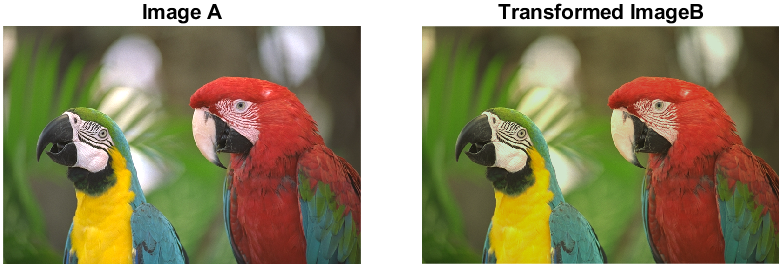
\includegraphics[width=1\textwidth]{KodimTransformed.png}
    \centering
    \caption{Tranformation of Kodim23b to color match Kodim23a}
    \label{fig:KodimTransform}
\end{figure}

\begin{figure}[!h]
    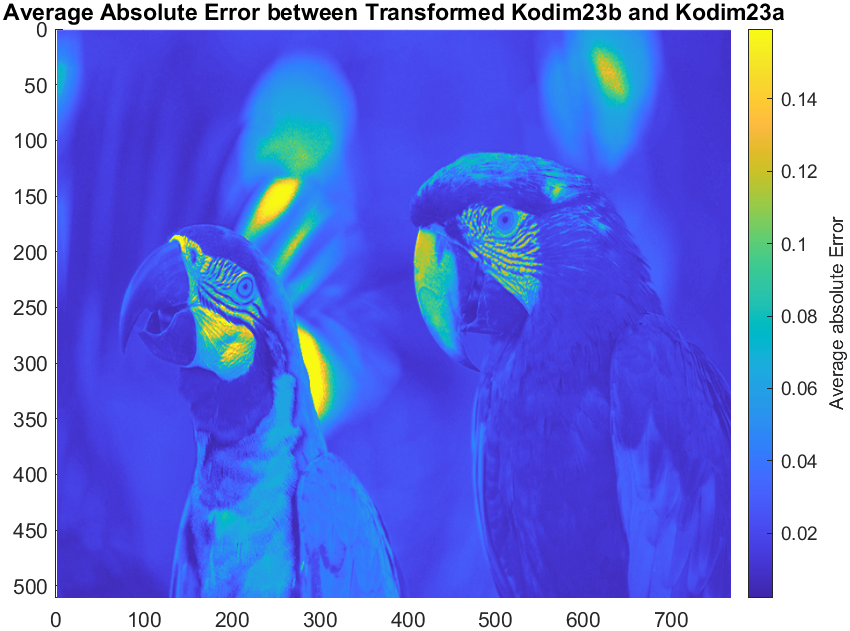
\includegraphics[width=1\textwidth]{KodimTransformedAAE.png}
    \centering
    \caption{Average Absolute error between Kodim23a and the transformed Kodim23b}
    \label{fig:KodimAAE}
\end{figure}
